\documentclass[a4paper,10pt]{report}

\usepackage{url}
\usepackage{graphicx}
\usepackage{verbatim}
\usepackage[usenames,dvipsnames]{color}
\usepackage{listings}
\usepackage{pifont}
\usepackage{bibentry}

% This looks better than CM
\usepackage{palatino}
\usepackage[margin=1.5in]{geometry}

% Colors
\definecolor{Blue}{rgb}{0,0,1}
\definecolor{Red}{rgb}{1,0,0}

% frequent acronyms, abbreviations, aliases, etc.
\newcommand{\ascii}{\textsc{ascii}}
\newcommand{\css}{\textsc{css}}
\newcommand{\eg}{\textit{e.g.}}
\newcommand{\gc}{\textsc{gc}}
\newcommand{\gnu}{\textsc{gnu}}
\newcommand{\ie}{\textit{i.e.}}
\newcommand{\lca}{\textsc{lca}}
\newcommand{\libxml}{libxml}
\newcommand{\no}{Newick order}
\newcommand{\nutils}{Newick Utilities}
\newcommand{\nw}{Newick}
\newcommand{\pdf}{\textsc{pdf}}
\newcommand{\phylip}{\textsc{phylip}}
\newcommand{\stderr}{standard error}
\newcommand{\stdin}{standard input}
\newcommand{\stdout}{standard output}
\newcommand{\svg}{\textsc{svg}}
\newcommand{\unix}{\textsc{Unix}}
\newcommand{\xml}{\textsc{xml}}

% names of programs
\newcommand{\clade}{\texttt{nw\_clade}}
\newcommand{\condense}{\texttt{nw\_condense}}
\newcommand{\display}{\texttt{nw\_display}}
\newcommand{\distance}{\texttt{nw\_distance}}
\newcommand{\duration}{\texttt{nw\_duration}}
\newcommand{\ed}{\texttt{nw\_ed}}
\newcommand{\gen}{\texttt{nw\_gen}}
\newcommand{\labels}{\texttt{nw\_labels}}
\newcommand{\match}{\texttt{nw\_match}}
\newcommand{\nwindent}{\texttt{nw\_indent}} % \indent already exists
\newcommand{\order}{\texttt{nw\_order}}
\newcommand{\prune}{\texttt{nw\_prune}} 
\newcommand{\reroot}{\texttt{nw\_reroot}}
\newcommand{\rename}{\texttt{nw\_rename}}
\newcommand{\support}{\texttt{nw\_support}}
\newcommand{\sched}{\texttt{nw\_sched}}
\newcommand{\stats}{\texttt{nw\_stats}}
\newcommand{\topology}{\texttt{nw\_topology}}
\newcommand{\trim}{\texttt{nw\_trim}}

% Arbitrary-size horizontal rules - good for titles
\newcommand{\Hrule}[1]{\rule{\linewidth}{#1}}

\begin{document}
\nobibliography*

\begin{titlepage}
\begin{center}
\Hrule{0.5mm} \\[0.8cm]
{\Huge Newick Utilities Tutorial} \\[0.5cm]
Version 1.3.5 -- \today \\
\medskip
Thomas Junier \texttt{thomas.junier@unige.ch} \\
Computational Evolutionary Genomics Group \\
Department of Genetic Medicine and Development \\
University of Geneva, Switzerland \\
\ding{91} \ding{91} \ding{91} \\
Swiss Institute of Bioinformatics \\
\medskip
\url{http://cegg.unige.ch/newick_utils}
\Hrule{0.5mm}
\\[2cm]
\includegraphics{title_svg.pdf}
\end{center}
\end{titlepage}

\tableofcontents


\chapter{Introduction}

The \nutils{} are a set of \unix{} shell programs for working with Newick-formatted phylogenetic trees. Their main features are:
\begin{itemize}
 \item they require no user interaction.\footnote{Why this is a good thing is not the focus of this document: I shall assume that if you are reading this, you already know when a command-line interface is better than an interactive interface.}
 \item they can work on any number of trees at a time\footnote{Strictly speaking, a few applications are limited to one input tree because working on more than one is not practical}
 \item they perform reasonably well with large trees
 \item they are implemented as filters
\end{itemize}
They are not tools for \emph{making} phylogenies. Rather, they are for working with existing ones, by which I mean manipulating the tree or extracting information from it: rerooting, simplifying, extracting subtrees, printing branch lengths and distances, etc - a glance at the table of contents of this document should give you an idea.

Each of the programs performs one task (with some variants). For example, here is how you would reroot a series of phylograms contained in file \texttt{mytrees.nw} using node \texttt{Dmelano} as outgroup:

\begin{verbatim}
$ nw_reroot mytrees.nw Dmelano
\end{verbatim} 
Now, you might want to make cladograms from the rerooted trees. Program \topology{} does the job, and since the utilities are filters, you can do it in a single command:
\begin{verbatim}
$ nw_reroot mytrees.nw Dmelano | nw_topology -
\end{verbatim}
As you can see, it is straightforward to pipe \nutils{} together, and of course they can be mixed freely with any other shell tool (see e.g. \ref{sct_counting_leaves}).

This document is organized as follows: chapter \ref{chap_general} discusses common features of the \nutils, chapter \ref{chap_simple} shows examples of simple tasks, and chapter \ref{chap_adv} has examples of more advanced tasks. 




\chapter{General Remarks}
\label{chap_general}

The following applies to all programs in the \nutils{} package.

\section{Help}
\label{sct_help}

All programs print a help message if passed option \texttt{-h}. Here are the
first 25 lines of \nwindent{}'s help, which you obtain by typig
\verb+nw_indent -h+:
\begin{samepage}
\verbatiminput{general_1_txt.out}
\end{samepage}
The help page describes the program's purpose, its input and output, and its
options, in a format reminiscent of \unix{} manpages. It also shows a few
examples. All examples can be tried out using files in the \texttt{data}
directory.

\section{Input}
\label{sct_input}

Since the \nutils{} are for working with trees, it should be no surprise
that the main input is a file containing Newick trees. The trees must be in
Newick format, which is one of the most widely used and uderstood formats. A
complete description can be found at
\url{http://evolution.genetics.washington.edu/phylip/newicktree.html}.

The input file is always the first argument to the program (after any options).
It may be a file stored in a:w filesystem, or \stdin{}. In the latter case, the
filename is replaced by a '\texttt{-}' (dash):
\begin{samepage}
\begin{verbatim}
$ nw_display mytrees.nw
\end{verbatim}
is the same as
\begin{verbatim}
$ cat mytrees.nw | nw_display -
\end{verbatim}
\end{samepage}
Of course the second form is only really useful when chaining several programs into pipelines.

\subsection{Multiple Trees in Input}

The input file can contain one or more trees, preferably one tree per
line\footnote{It may also work if the trees are formatted differently, but the
programs were only tested on input files with one tree per line.}. The task
will be performed on each tree in the input. So if you need to reroot 1,000
trees on the same outgroup, you can do it all in a single step (see
\ref{sct_reroot}). 

\section{Output}
\label{sct_output}

All output is printed on \stdout{} (error messages go to \stderr). The \nutils{}
either print trees or information about trees. In the first case, the output is
also Newick. In the second case, the format depends on the program, but it is
always text (\textsc{ascii} graphics, \svg, numeric data, textual data, etc.).

\section{Options}
\label{sct_options}

Options change program behaviour and/or allow extra arguments to be passed.
They are all passed on the command line, before the mandatory argument(s),
using a single letter preceded by a dash - in the usual \unix{} way. There are
no mandatory control files, although some tasks require additional files (\eg{}
\ref{sct_display_svg_css}). For example, we saw above that \display{} produces
graphs. By default the graph is \ascii{} graphics, but with option \texttt{-s},
the program produces \svg:
\begin{verbatim}
$ nw_display -s sometree.nw
\end{verbatim}
All options are described in the program's help page (see \ref{sct_help}).



\chapter{Simple Tasks}
\label{chap_simple}


\section{Displaying Trees}
\label{sct_display}

Perhaps the simplest and most common operation on a \nw{} tree is just to look
at it. The \nw{} format is not very easy to understand for us humans, so we
have to produce a graphical representation from it. This is the purpose of the
\display{} program. 

\subsection{As Text}
\label{sct_display_text}

At its simplest, \display{} just outputs a text graph. Here is a
Newick-formatted tree in file \texttt{catarrhini}:
\verbatiminput{catarrhini}
And here is the same tree shown with \display{}:
\verbatiminput{display_1_txt.cmd}
\begin{samepage}
\verbatiminput{display_1_txt.out}
\end{samepage}
That's pretty low-tech compared to interactive, colorful graphical displays,
but if you use the shell a lot (like I do), you may find it useful.

You can use option \texttt{-w} (``width'') to set the number of columns
available for display (the default is 80):

\verbatiminput{display_2_txt.cmd}
\begin{samepage}
\verbatiminput{display_2_txt.out}
\end{samepage}

\subsection[As SVG]{As Scalable Vector Graphics}
\label{sct_display_svg}

First, a disclaimer: there are dozens of tools for viewing trees out there, and
I'm not interested in competing with them. The reasons why I added \svg{}
capabilities to \display{} were:
\begin{itemize}
\item I wanted to be able to produce reasonably good graphics even if no other
tool was at hand
\item I wanted to be sure that large trees could be rendered\footnote{I have had serious problems
visualising trees of more than 1,000 leaves using some popular software I will
not name here - either it was painfully slow, or it simply crashed}
\end{itemize}
To produce \svg, pass option \texttt{-s}:
\begin{verbatim}
$ nw_display -s catarrhini > catarrhini.svg
\end{verbatim}
Now you can visualize the result using any \svg-enabled tool (all good Web browsers can do it), or convert it to another format with, say \texttt{rsvg} or Inkscape. The following \pdf{} image was produced like this:

\begin{verbatim}
$ inkscape -f catarrhini.svg -A catarrhini.pdf
\end{verbatim}

\begin{center}
 \includegraphics{display_3_svg.pdf}
\end{center}
All \svg{} images shown in this document were produced in the same way. In the
rest of this document we will usually skip the redirection into an \svg{} file
and omit the \svg{}-to-\textsc{pdf} conversion step.

The \svg{} produced by \display{} is designed to be easy to edit
in an interactive editor like Inkscape (\url{http://www.inkscape.org}): the
tree edges are in one group, and the text in another. So it is easy to change
the line properties of the edges, or the font family of the text, for example
(you can also do this from \display{} using a \css{} map, see
\ref{sct_display_svg_css}).

There are many options for \svg{} graphs. First, you can make radial trees,
using option \texttt{-r} 
\verbatiminput{display_4_svg.cmd}
You already know \texttt{-w}, except that for \svg{} the value is in pixels instead of columns. 

\begin{center}
\includegraphics{display_4_svg.pdf}
\end{center}

\subsubsection{Scale Bar}

If the tree is a phylogram, \display{} prints a scale bar.\footnote{The
positioning of the scale bar is a bit crude, especially for radial trees. This
is mainly because of the "\svg{} string length curse", that is, the
impossibility of finding out the length of a text string in \svg. This means it
is hard to ensure the scale bar will not overlap with a node label, unless one
places it far away in a corner, which is what I do for now. An improvement of
this is on my TODO list.} Its units can be specified with option \texttt{-u},
the default is substitutions per site. To suppress the scale bar, pass the
\texttt{-S} switch.

\subsubsection{Using CSS}
\label{sct_display_svg_css}

You can modify node style using \css. This is done by specifying a
\textit{\css{} map}, which is just a text file that says which style should be
applied to which node. If file \texttt{css.map} contains the following
\begin{quote} \verbatiminput{css.map} \end{quote} we can apply the style map to
the tree above:

\verbatiminput{display_5_svg.cmd}

\begin{center}
 \includegraphics{display_5_svg.pdf}
\end{center}

The syntax of the \css{} map file is as follows. Each line describes one style
and the set of nodes to which it applies. A line contains elements separated by
whitespace (whitespace between quotes does not count). The first element of the
line is the style, and it is a snippet of \css{} code. The second element is
either \texttt{Clade} or \texttt{Individual} and states whether the following
nodes are to be treated individually or as a clade. The next element(s) are
node labels and specify the nodes to which the style must be applied: if the
second element was \texttt{Clade}, the program finds the last common ancestor
of the nodes and applies the style to that node and all its descendants. If the
second element was \texttt{Individual}, then the style is only applied to the
nodes themselves.

In our example, the first line in \texttt{css.map} says that the style
\texttt{stroke:red} must be applied to the \texttt{Clade} defined by
\texttt{Macaca} and \texttt{Cercopithecus}, which consists of these two nodes,
their ancestor \texttt{Cercopithecinae}, and \texttt{Papio}. The \texttt{Clade}
keyword can be abbreviated to \texttt{C}, as in the next line. Line 2
prescribes that style \texttt{stroke:\#fa7} (an \svg{} hexadecimal color
specification) must be applied to the clade defined by \texttt{Homo} and
\texttt{Hylobates}, which consists of these two nodes, their last common
ancestor (unlabeled), and all its descendants (that is, \texttt{Homo},
\texttt{Pan}, \texttt{Gorilla}, \texttt{Pongo}, and \texttt{Hylobates}, as well
as the inner nodes \texttt{Hominini}, \texttt{Homininae} and
\texttt{Hominidae}). Line 3 says that the style \texttt{stroke:green} is to be applied to nodes \texttt{Colobus} and \texttt{Cercopithecus}, and only these nodes - not to the clade that they define. 
Line 4 says that the clade defined by \texttt{Homo} and
\texttt{Pan} should receive style \texttt{stroke-width:2;~stroke:blue} - note
that the quotes have been removed: they are not part of the style, rather they
allow us to improve readability by adding some whitespace.

The style of an inner clade overrides that of an outer clade, \textit{e.g.},
although the \texttt{Homo} - \texttt{Pan} clade is nested inside the
\texttt{Homo} - \texttt{Hylobates} clade, it has its own style (blue, wide
lines) which overrides the containing clade's style (pinkish with normal
width).

Also, note that \texttt{Individual} overrides \texttt{Clade}, which is why
\texttt{Cercopithecus} is green even though it belongs to a red clade.

The \texttt{Clade} and \texttt{Individual} keywords are not case-sensitive and
can be abbreviated - in fact only the first letter counts.

Styles can also be applied to labels. Option \texttt{-l} specifies the leaf
label style, option \texttt{-i} the inner node label style, and option
\texttt{-b} the branch length style. For example, the following tree, which was
produced using defaults, could be improved a bit:

\verbatiminput{display_6_svg.cmd}
\begin{center}
  \includegraphics{display_6_svg.pdf}
\end{center}

\noindent{}Let's remove the branch length labels, reduce
the vertical spacing, reduce the size of inner node labels (bootstrap values),
and write the leaf labels in italics, using a font with serifs:
\verbatiminput{display_7_svg.cmd}
\begin{center}
  \includegraphics{display_7_svg.pdf}
\end{center}
Option \texttt{-v} specifies the vertical spacing, in pixels, between two
successive leaves (the default is 40). Option \texttt{-b} sets the style of
branch labels, option \texttt{-l} sets the style of leaf labels, and option
\texttt{-i} sets the style of inner node labels. Note that we did not
\emph{discard} the branch lengths (we could do this with \topology), because
doing so would reduce the tree to a cladogram. Instead, we set their \css{}
style to \texttt{opacity:0} (\texttt{visibility:hidden} also works).

\subsection{Ornaments}

Ornaments are arbitrary snippets of \svg{} code that are displayed at specified
node positions. As for \css, this is done with a map. The ornament map has the
same syntax as the \css{} map, except that you specify \svg{} elements rather
than \css{} styles. The \texttt{Individual} keyword means that all nodes are
sport the ornament, while \texttt{Clade} means that only the clade's \lca{}
must be adorned. The ornament is translated in such a way that its (0,0)
coordinate corresponds to the position of the node.

The following file, \texttt{ornament.map}, instructs to draw a red circle with
a black border on \texttt{Homo} and \texttt{Pan}, and a cyan circle with a blue
border on the root of the \texttt{Homo} - \texttt{Hylobates} clade. The \svg{}
is enclosed in double quotes because it contains spaces - note that single
quotes are used for the values of \xml{} attributes. The ornament map is
specified with option \texttt{-o}:
\begin{quote}
 \verbatiminput{ornament.map}
\end{quote}
\verbatiminput{display_8_svg.cmd}
\begin{center}
 \includegraphics{display_8_svg.pdf}
\end{center}
Ornaments and \css{} can be combined:
\verbatiminput{display_9_svg.cmd}
\begin{center}
 \includegraphics{display_9_svg.pdf}
\end{center}

\subsubsection{Example: Mapping GC Content}

In a study of human rhinoviruses, I have produced a phylogenetic tree. I have
also computed the \gc{} content of all sequences, and mapped it into a color
map that goes from {\color{Blue} blue} (33.3\%) to {\color{Red} red} (44.5\%).
\texttt{b2r.map}. Then:

\verbatiminput{display_10_svg.cmd}
\includegraphics{display_10_svg.pdf}
\bigskip{}

\noindent{}As we can see, the high-\gc{} sequences are all found in the same main clade.

\subsubsection{Multiple SVG Trees}

Like all \nutils, \display{} can handle multiple trees, even in \svg{} mode.
The best way to do this is not evident: one can generate one file per tree (but
then we break the rule that every program is a filter and so writes to standard
output), or one can put all the trees in one \svg{} document (but then we have
to impose tiling or some other arrangement), or one can just output one \svg{}
document after another. This is what we do (this may change in the future). So
if you have many trees in document \texttt{forest.nw}, you can say:
\begin{quote}
\verb+$ nw_display -s forest.nw > forest_svg+
\end{quote}
But \texttt{forest\_svg} isn't valid \svg{} -- it is a concatenation of many \svg{} documents. You can just extract them into individual files with \texttt{csplit}:
\begin{quote}
\verb+$ csplit -sz -f tree_ -b '%02d.svg' forest_svg '/<?xml/' {*}+
\end{quote}
This will produce one \svg{} file per tree in \texttt{forest.nw}, named \texttt{tree\_01.svg}, \texttt{tree\_02.svg}, etc.

\subsection{Options not Covered}

\display{} has many options, and we will not describe them all here - all of
them are described when you pass option \texttt{-h}. They include support for
clickable images (with URLs to arbitrary Web pages), setting the scale bar
units, changing the root length, etc. 



\section{Indenting}
\label{sct_indent}

\nwindent{} reformats the \nw{} on several lines, with one node per line,
nodes of the same depth in the same column, and children nodes to the right of
their parent. This shows the structure more
clearly than the compact form, but since whitespace is ignored in the Newick
format\footnote{except between quotes}, the
indented form is still valid. For example, this is a tree in compact form, in
file \texttt{falconiformes}:
\verbatiminput{falconiformes}
And this is the same tree, indented:
\verbatiminput{indent1_nw.cmd}
\verbatiminput{indent1_nw.out}
The structure is much more clear, it is also relatively easy to edit manually
in a text editor - while still being valid \nw.

Another advantage of indenting is that it is resistant to certain errors
which would cause \display{} to fail.\footnote{This is
because indenting is a purely lexical process, hence it does not need a
syntactically correct tree.} For example, there is an error in this tree:
\verbatiminput{falconiformes_error}
yet it is hard to spot, and trying \display{} won't help as it will abort with a
parse error. With \nwindent{}, however, you can at least look at the tree:
\verbatiminput{indent4_nw.out}
While the error is not exactly obvious, you can at least view the Newick. It turns out there is a comma missing after \texttt{Sagittarius}.

The indentation can be varied by supplying a string (option \texttt{-t}) that
will be used instead of the default (which is two spaces). If you want a deeper
indentation, you could say this:
\verbatiminput{indent2_nw.cmd}
\verbatiminput{indent2_nw.out}
Option \texttt{-t} can also be used to highlight indentation:
\verbatiminput{indent3_txt.cmd}
\verbatiminput{indent3_txt.out}
Now the indentation levels are easier to see, but at the expense of the tree no
longer being valid \nw.

Finally, option \texttt{-c} ("compact") does the reverse: it removes all
indentation and produces a compact tree. You can use this when you want to
produce a compact Newick file after editing. For example, using Vim, after
loading a newick tree I do 
\begin{quote}
\verb+gg!}nw_indent -+
\end{quote}
to indent the file, then I edit it, then compact it again:
\begin{quote}
\verb+gg!}nw_indent -c -+
\end{quote}




\section{Rooting and Rerooting}
\label{sct_reroot}

Rooting transforms an unrooted tree into a rooted one, and rerooting changes a rooted tree's root. Some tree-building methods produce rooted trees (e.g., \textsc{UPGMA}), others produce unrooted ones (neighbor-joining, maximum-likelihood). 

The Newick format is implicitly rooted, in the sense that there is a 'top' node from which all other nodes descend. Some applications regard a tree with a trifuraction at the top node as unrooted. 

One way of (re)rooting a tree is to specify an \textit{outgroup}. In the simplest case, this is a single leaf. The root is then placed in such a way that one of its children is the outgroup, while the other child is the rest of the tree (sometimes known as the \textit{ingroup}). 

Consider the following primate tree, \texttt{simiiformes\_wrong}:

\includegraphics{reroot_1og_orig_svg.pdf}

\noindent{}It is wrong because \texttt{Cebus}, which is a New World monkey (capuchin), should be the sister group of all the rest (Old World monkeys and apes, technically Catarrhini), whereas it is shown as the sister group of the macaque-colobus family, Cercopithecidae. We can correct this by re-rooting the tree using \texttt{Cebus} as outgroup:
\verbatiminput{reroot_1og_corr_svg.cmd}
which produces:
\includegraphics{reroot_1og_corr_svg.pdf}

The outgroup does not need to be a single leaf. The following tree is wrong for the same reason as the one before, except that is has three New World monkey species instead of one, and they appear as a clade (Platyrrhini) in the wrong place:

\includegraphics{reroot_3og_orig_svg.pdf}

\noindent{}We can correct this by specifying the New World monkey clade as outgroup:

\verbatiminput{reroot_3og_result_svg.cmd}

\includegraphics{reroot_3og_result_svg.pdf}

\noindent{}Note that I did not include all three New World monkeys, only \texttt{Cebus} and \texttt{Allouatta}. This is because it is always possible to define a clade using only two leaves. The result would be the same if I had included all three, though. You can use inner labels too, if there are any:
\begin{verbatim}
$ nw_reroot simiiformes_wrong_3og Platyrrhini
\end{verbatim}
will reroot in the same way (not shown). Beware that inner labels are often used for support values (as in bootstrapping), which are generally not useful for defining clades.

\section{Extracting Labels}
\label{sct_labels}

To get a list of all labels in a tree, use \labels:

\verbatiminput{labels_xpl1_txt.cmd}
\verbatiminput{labels_xpl1_txt.out}

\noindent{}The labels are printed out in post-order. To get rid of internal labels, use \texttt{-I}:

\verbatiminput{labels_xpl2_txt.cmd}
\verbatiminput{labels_xpl2_txt.out}

\noindent{}Likewise, you can use \texttt{-L} to get rid of leaf labels (not shown). Finally, if you use \texttt{-t} the labels are printed on a single line, separated by tabs (for some reason the tabs show as spaces here, I think this is an effect of \LaTeX{}'s \verb+\verbatiminput{}+):

\verbatiminput{labels_xpl3_txt.cmd}
\verbatiminput{labels_xpl3_txt.out}

\subsection{Counting Leaves in a Tree}
\label{sct_counting_leaves}

A simple application of \labels{} is a leaf count:

\verbatiminput{labels_xpl4_txt.cmd}
\verbatiminput{labels_xpl4_txt.out}





\section{Extracting Subtrees}
\label{sct_subtrees}

You can extract a clade from a tree with \clade. You pass it a number of
labels; it then computes the \lca{} of those labels, and prints out the subtree
rooted at the \lca, in \nw (see Appendix \ref{sct_define_clades} for more on
how to specify clades).


Say you want to extract the 





\chapter{Advanced Tasks}
\label{chap_adv}

The tasks presented in this chapter are more complex than that of chapter
\ref{chap_simple}, and generally involve many \nutils{} as well as other
programs.

\section{Higher Level Trees from Lower Level Ones}
\label{sct_higher_lvl}



\section{Finding Recombination Breakpoints}
\label{sct_bootscanning}

Bootscanning is a technique for finding recombination breakpoints in a
sequence. The original procedure \cite{Salminen_1995} uses the bootstrap value
of competing topologies as a criterion, the procedure shown below uses the
patristic distance (\ie, distance along the tree) according to the most likely
tree, and is thus not strictly speaking a bootscan but a distance
plot.\footnote{Thanks to Heiko Schmidt for pointing this out.} It involves
aligning the sequence of interest (called \emph{query} or \emph{reference})
with related sequences (including the putative recombinant's parents) and
computing phylogenies locally over the alignment.  Recombination is expected to
cause changes in topology.  The tasks involved are shown below:
\begin{enumerate}
\item align the sequences $\rightarrow$ multiple alignment
\item slice the multiple alignment $\rightarrow$ slices
\item build a tree for each slice $\rightarrow$ trees
\item extract distance from query to other sequences (each tree) $\rightarrow$ tabular data
\item plot data $\rightarrow$ graphics
\end{enumerate}
The distribution contains a script, \texttt{src/bootscan.sh}, that performs the whole process. Here is an example run:
\begin{verbatim}
$ bootscan.sh HRV_3UTR.dna HRV-93 CL073908
\end{verbatim}
where \texttt{HRV\_3UTR.dna} is a FastA file of (unaligned) sequences, \texttt{HRV-93} is the outgroup, and \texttt{CL073908} is the query.  Here is the result:

\begin{centering}
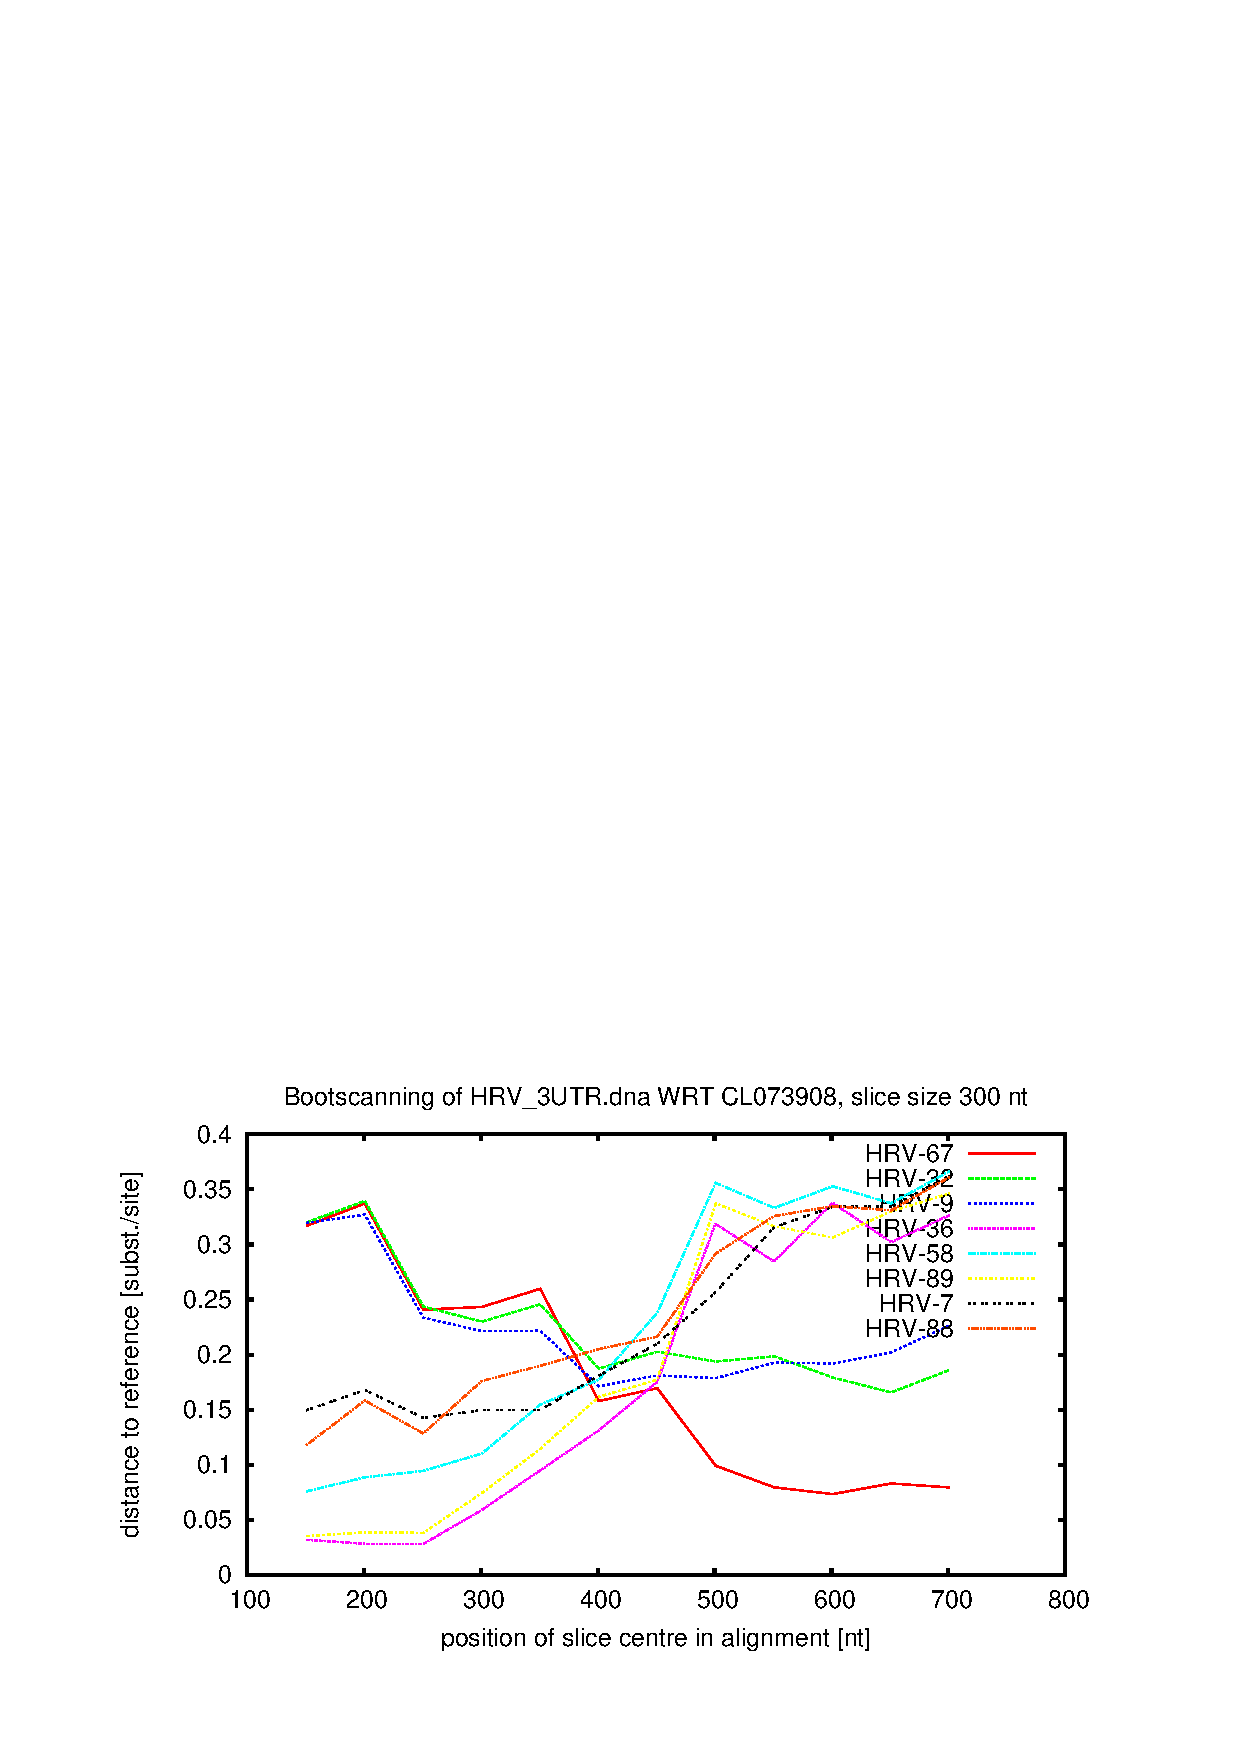
\includegraphics[width=\textwidth]{bootscan_1.pdf}
\end{centering}

\smallskip{}
\noindent{}until position 450 or so, the query sequence's nearest relatives (in
terms of substitutions/site) are \texttt{HRV-36} and \texttt{HRV-89}. After
that point, it is \texttt{HRV-67}. This suggests that there is a recombination
breakpoint near position 450.

The script uses \reroot{} to reroot the trees on the outgroup, \clade{} and
\labels{} to get the labels of the ingroup, \distance{} to extract the distance
between the query and the other sequences, as well as the usual \texttt{sed}, \texttt{grep}, etc. The plot is done with gnuplot.


\section{Number of nodes vs. Tree Depth}
\label{clades_vs_depth}

A simple measure of a tree's shape can be obtained by computing the number of
nodes as a function of depth. Consider the following trees:

\smallskip{}
\begin{tabular}{ccc}
\texttt{star} & \texttt{balanced} & \texttt{short\_leaves} \\
\hline \\
\includegraphics{clades_vs_depth_1_svg.pdf} &
\includegraphics{clades_vs_depth_2_svg.pdf} &
\includegraphics{clades_vs_depth_3_svg.pdf}
\end{tabular}
\smallskip{}

\noindent{}they have the same depth and the same number of
leaves.  But their shapes are very different, and they tell different
biological stories. If we assume that they are clock-like (i.e., that the
mutation rate is constant over the whole tree), \texttt{star.nw} shows an early
radiation, \texttt{short\_leaves.nw} shows two stable branches ending in
recent branching, while \texttt{balanced.nw} shows branching spread over time.

The nodes-vs-depth graphs for these trees are as follows: \\
\includegraphics[width=12cm]{star.pdf} \\
\includegraphics[width=12cm]{balanced.pdf} \\
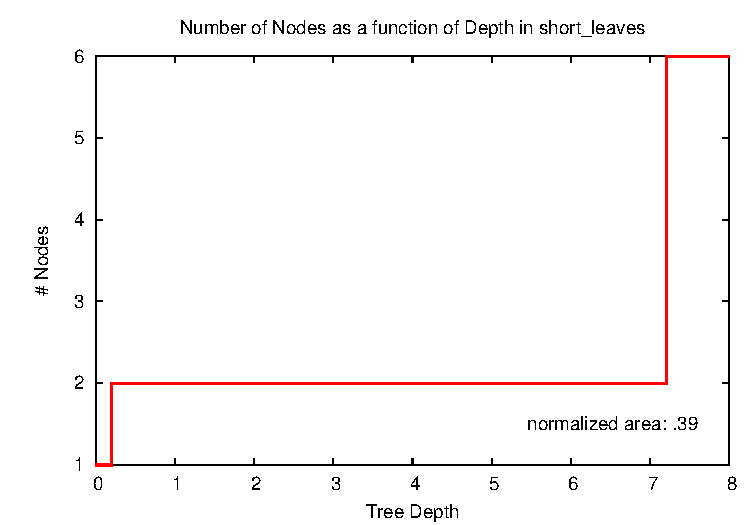
\includegraphics[width=12cm]{short_leaves.pdf} \\

The graphs show the (normalized) area under the curve: it is close to 1 for star-like trees, close to 0 for trees with very short leaves, and intermdiary for more balanced trees.

The images were made with the \texttt{bootscan.sh} script (in directory \texttt{src}), in the following way:
\begin{verbatim}
$ nodes_vs_clades.sh star.nw 40
\end{verbatim}
where 40 is just the sampling density (how many points to take on the $x$
axis). The script uses \distance{} to get the tree's depth, \ed{} to sample the number of nodes at a given depth, and \nwindent{} to count the leaves, plus the usual \texttt{awk} and friends. The plot is done with gnuplot.



\lstset{
	language=Python,
	basicstyle=\ttfamily,
	keywordstyle=\color{NavyBlue},
	stringstyle=\color{OliveGreen},
	commentstyle=\color{red},
	frame=single,
	frameround=tttt,
	framexleftmargin=8mm,
	numbers=left
}

\chapter{Python Bindings}
\label{chap_python_lib}

This chapter shows how you can use the \nutils{}'s functionalities in Python
programs. While the \nutils{} are written in C, the \texttt{ctypes}
module\footnote{Available in Python 2.5 and up} makes it easy to access them
from Python, and the distribution contains a module, \texttt{newick\_utils.py},
that provides an object-oriented interface to the underlying C code.

Let's say we want to add a utility that prints simple statistics about trees,
like the number of nodes, the depth, whether it is a cladogram or a phylogram,
etc. We will call it \texttt{nw\_info.py}, and we'll pass it a \nw{}
file on standard input, so the usage will be something like:

\begin{verbatim}
$ nw_info.py < data/catarrhini
\end{verbatim}

\noindent{}The overall structure of this program is simple: iteratively read
all the input trees, and do something with each of them:

\begin{lstlisting}
from newick_utils import *

for tree in Tree.parse_newick_input():
    pass # process tree here!
\end{lstlisting}

\noindent{}Line 1 imports definitions from the \texttt{newick\_utils.py}
module. Line 2 is the main loop: the \texttt{Tree.parse\_newick\_input}
reads standard input and yields an instance of class \texttt{Tree} for each
Newick string. We can now work with it, using methods of class \texttt{Tree} or adding our own:

\lstinputlisting{../src/nw_info.py}

\noindent{}When we run the program, we get:

\verbatiminput{python_1_txt.cmd}
\verbatiminput{python_1_txt.out}

As you can see, most of the work is done by methods called on the \texttt{tree}
object, such as \texttt{get\_leaf\_count} which (surprise!) returns the number
of leaves of a tree. But since there is no method for coounting polytomies, we
added our own function, \texttt{count\_polytomies}, which takes a \texttt{Tree}
object as argument.

Detailed information about all classes and methods is found in file
\texttt{newick\_utils.py}.


\appendix

\chapter{Defining Clades by their Descendants}
\label{sct_def_clades}

When you need to specify a clade using the \nutils{}, you either give the label
of the clade's root, or the labels of (some of) its descendants. Since inner
node rarely have labels (or worse, have unuseable labels like bootstrap support
		values), you will often need to specify clades by their
descendants.

Consider the following tree:

\begin{center}
\includegraphics{reroot_1og_corr_svg.pdf} 
\end{center}

Suppose we want to specify the Hominoidea clade - the apes. It is the clade
that contains \texttt{Homo}, \texttt{Pan} (chimps), \texttt{Gorilla},
     \texttt{Pongo} (orangutan), and \texttt{Hylobates} (gibbons). The clade is
     not labeled in this tree, but this list of labels defines it without
     ambiguity. In fact, we can define it unambiguously using just
     \texttt{Hylobates} and \texttt{Homo} - or \texttt{Hylobates} and any other
     label. The point is that \emph{you never need more than two labels to
     unambiguously define a clade}.

You cannot choose any two nodes, however: the condition is that the last
common ancestor of the two nodes be the root of the desired clade.

\section{Why not just use node numbers?}

Some applications atribute numbers to all inner nodes and allow users to specify clades by refering to this number. Such a scheme is not workable when one has many input trees, however, because tere is no guarantee that the same clade (assuming it is present) will have the same number.


\chapter{Newick order}
\label{newick_order}

There are many ways of visiting a tree. One can start from the root and
proceed to the leaves, or the other way around. One can visit a node before
its children (if any), or after them. Unless specified otherwise, the
\nutils{} process trees as they appear in the \nw{} data. That is, for
tree \texttt{(A,(B,C)d)e;} the order will be A, B, C, d, e.

This means that a child always comes before its parent, and in particular,
that the root comes last. This is known as reverse post-order traversal, but
we'll just call it "\nw{} order".


\chapter{Installing the \nutils}

\section{From source}

I have tested the \nutils{} on various distributions of Linux, as well as on
Mac OS X and Cygwin\footnote{I use Linux as a main development platform.
Although I try my best to get the package to compile on Macs and Cygwin, I don't
always succeed.}. On Linux, chances are you already have development tools
preinstalled, but some distributions (\eg, Ubuntu) do not install \textsc{gcc},
etc. by default. Check that you have \textsc{gcc}, Bison, Flex, and the
\textsc{gnu} autotools, including Libtool. The same goes for Cygwin. On MacOS X,
you need to install XCode (\url{http://developer.apple.com/tools/xcode}).
Here are the versions I use (as reported by passing \texttt{--version} to the
program):

\medskip
\begin{tabular}{lll}
Autoconf	& autoconf (GNU Autoconf) & 2.63 \\
Automake	& automake (GNU automake) & 1.11.1 \\
Bison  		& bison (GNU Bison) 			& 2.4.1 \\ 
Flex			& flex 										& 2.5.35 \\
GCC 			& gcc (GCC) 							& 4.4.1 20090725 (Red Hat 4.4.1-2) \\
Libtool		& ltmain.sh (GNU libtool) & 2.2.6b \\
Make			& GNU Make 								& 3.81
\end{tabular}
\medskip

\noindent{}The package uses the \textsc{gnu} autotools, like many other open source
software packages. So all you need to do is the usual
\begin{verbatim}
$ tar xzf newick-utils-x.y.z.tar.gz
$ cd newick-utils-x.y.z
$ ./configure
$ make
$ make check
# make install
\end{verbatim}
The \texttt{make check} is optional, but you should try it anyway. Note that
the \gen{} test may fail - this is due to differences in pseudo-random number
generators, as far as I can tell.


\section{As binaries}

Since version 1.1, there are also binary distribution for some platforms. The
name of the archive matches \texttt{newick-utils-<version>-<platform>.tar.gz}.
All you need to do is:

\begin{verbatim}
$ tar xzf newick-utils-<vesion>-<platform>.tar.gz
$ cd newick-utils-<vesion>-<platform>
\end{verbatim}

\noindent{}The binaries are in \texttt{src}. Testing may be less important than
when installing from source, but you can do it like this:

\begin{verbatim}
$ cd tests
$ for test in test*.sh; do ./$test; done 
\end{verbatim}

\noindent{}any failure will generate a \texttt{FAIL} message (which you could filter with \texttt{grep}, etc).  You can then copy/move the binaries wherever it suits you.



\bibliographystyle{plain}
\bibliography{references}

% \chapter{Axiomatic Construction of Rooted Trees}

Here is one way of considering rooted trees. We start with a set $N$, whose
elements we call \emph{nodes}.  We'll assume that $N \neq \emptyset$, because
empty trees are not very interesting. Then we introduce an irreflexive,
antisymmetric relation on $N$, noted $<$:
\begin{align}
n \nless n & & \forall \; n \in N & & \text{irreflexivity} \\
m < n \Rightarrow n \nless m &  & \forall \; m, n \in N & &  \text{antisymmetry}
\end{align}
In other words, $<$ is a binary relation on $N$ such that no node is
related to itself, and if node $n$ is related to $m$, then $m$ is \emph{not}
related to $n$. If $m < n$, we say that $m$ is a \emph{parent} of $n$.

Now we introduce axioms that produce rooted trees.
\begin{axiom}
There exists a node that has no parent:
\[ \exists \; r \in N \; | \; n \nless r \qquad \forall \; n \in N \]
\end{axiom}

\begin{axiom}
There is only one node that has no parent. Let $S = \{x \in N\,|\, n \nless x \; \forall \; n \in N \}$ be the set of parent-less nodes of $N$. Then:
\[ r, s \in S \quad \Rightarrow \quad r = s \qquad \forall \;r, s \in N \]
\end{axiom} 

The unique parent-less node of $N$ is called the \emph{root}.

\begin{axiom}
Every node except the root has a parent.
\end{axiom} 

\begin{axiom}
No node has more than one parent.
\end{axiom} 

We can now speak of \emph{the} parent of node $n$ (unless $n$ is the root), and we will note it $\mathrm{par}(n)$.


% \chapter{Some Properties of Trees}
\label{sct_defining_clades}

\begin{figure}[t]
\centering
\includegraphics{oriented_graph.png}
 % oriented_graph.png: 485x393 pixel, 300dpi, 4.11x3.33 cm, bb=0 0 116 94
 \caption{An oriented graph (not a tree!), with edge orientation shown as arrows. Two paths are highlighted (cyan and blue). The cyan path starts at node A and ends at node E. Nodes B, C, D, and E are reachable from A. Node C is the direct successor of B in the cyan path; in the blue path the direct successor of B is F. The segment highlighted in red is \emph{not} a path.}
 \label{fig_oriented_graph}
\end{figure}



In the following, $T$ will be a rooted tree. We'll recall that a tree (rooted or not) is a connected, acyclic graph. By choosing one node to be the root (which we'll note $R$), and orienting all edges away from the root, we get an oriented graph. A \textit{path} along such a graph is a sequence of nodes such that there is an edge between two successive nodes, and that these nodes are ordered in the sequence as they are in the edge. The first node in the path is called the \textit{start} of the path, and the last node is its \textit{end}. We speak of a path \textit{from} the start \textit{to} the end, equivalently we say that the end is \textit{reachable} from the start. The nodes in a path are ordered: if $a$ and $b$ are in a path, then either $a$ is reachable from $b$, or $b$ is reachable from $a$, or $a = b$; furthermore if $a$ is reachable from $b$, then $b$ is \textit{not} reachable from $a$. If an edge connects $a$ to $b$, then $b$ is the \textit{direct successor} of $a$, and $a$ is the \textit{direct predecessor} of $b$
See figure {\ref{fig_oriented_graph}.

Although paths are not sets, we will (somewhat abusively, perhaps) use set notation with paths, unless there is a risk of confusion. Thus is $P$ is a path and $n$ is a node, then $n \in P$ means that $n$ is ``in'' $P$  or ``belongs to'' $P$ (strictly speaking, $n$ is reachable from the start of $P$, and the end of $P$ is reachable from $n$).

Now a few definitions - these are mostly renamings of graph-theoretical concepts, to make them more intuitive for phylogenetic trees. 

\begin{dfn}
\label{def_ancestor}
Let $a$ and $b$ be two different nodes of $T$. We say that $a$ is an \textit{ancestor} of $b$, or (equivalently) that $b$ is a \textit{descendant} of $a$, if and only if there is a path from $a$ to $b$. 
\end{dfn}

\begin{dfn}
\label{def_parent}
Let $P$ be a path in $T$, and $a, b$ two nodes in $P$ such that $b$ is the direct successor of $a$. We will call $a$ the \textit{parent} of $b$. We can say \textit{the} parent (rather than \textit{a} parent) of $b$ because i) $a$ lies on the path from $R$ to $b$ (which is unique), and ii) only one node on any path can be another node's direct predecessor. We also see that any node's parent is also its ancestor (which shouldn't be too surprising\ldots), since $b$ is reachable from $a$
\end{dfn}

\begin{dfn}
\label{def_child}
Let $P$ be a path in $T$, and $a, b$ two nodes in $P$ such that $b$ is the direct successor of $a$. We say that $b$ is a \textit{child} of $a$.
\end{dfn}

Note that a node has exactly one parent, except the root which has none. A node can have zero or more children, but we rarely ever encounter nodes with a single child. A node with no children is called a \textit{leaf}.

\begin{dfn}
\label{def_lineage}
A path that starts from the root we call a \emph{lineage}. By the definition of a rooted tree, there is always a lineage to $n$ for any node $n$, and this lineage is unique. So we can unambiguously talk of \textit{the} lineage of $n$ to mean the path from $R$ to $n$. We say that a set $L$ of nodes form a lineage if there exists $n \in L$ such that the path from $R$ to $n$ contains all and only elements of $L$.
\end{dfn}

\begin{figure}[b]
 \centering
 \includegraphics{prop_tree.png}
  \caption{A rooted tree}
 \label{fig_app_tree_prop}
\end{figure}

\begin{prop}
\label{prop_lineage_ancestors_equivalence}
Let $n$ be a node of $T$, and $L$ its lineage. Then all ancestors of $n$ belong to $L$, and all nodes of $L$, except $n$ itself, are ancestors of $n$.
\end{prop}

\begin{proof}

$\Rightarrow$ Let $a$ be an ancestor of $n$. By definition \ref{def_ancestor}, there is a path from $a$ to $n$. By tree properties, there is a path from $R$ to $a$. Hence $a$ belongs to the path from $R$ to $n$, which is the lineage of $n$.
\end{proof}

\noindent{}$\Leftarrow$ Let $l \neq n$ be a node in $L$. Since $L$ is the path from $R$ to $n$, $n$ is reachable from $a$, and hence $a$ is an ancestor of $n$ by definition \ref{def_ancestor}.

\begin{dfn}
If $L$ and $M$ are lineages of $T$, then the \textit{intersection}
of $L$ and $M$, noted $L \cap M$, is the set of nodes that belong to both $L$ and $M$.
\end{dfn} 

\begin{lemma}
\label{lem_ancestors_in_lineage}
Let $n$ be a node of $T$, $L$ its lineage, and $l$ a node of $L$. Then $l$'s ancestors also belong to $L$.
\end{lemma}
\begin{proof}
If $l = n$ then the ancestors of $l$ are those of $n$, which belong to $L$ by proposition \ref{prop_lineage_ancestors_equivalence}. If $l \neq n$ then let $a$ be an ancestor of $l$. By definition \ref{def_ancestor}, $l$ is reachable from $a$. By proposition \ref{prop_lineage_ancestors_equivalence}, $l$ is an ancestor of $n$ and again $n$ is reachable from $l$. Therefore, $n$ is reachable from $a$, so $a$ is an ancestor of $n$, and so belongs in $L$.
\end{proof}

\begin{lemma}
Let $L$ and $M$ be lineages of $T$, and $q \in L \cap M, q \neq R$. Then $q$'s parent also belongs to $M \cap L$.
\end{lemma}
\begin{proof}
Call $p$ the parent of $q$. $p$ is an ancestor of $q$, and since $q$ belongs to $L$ (by hypothesis), $p$ belongs to $L$ by lemma \ref{lem_ancestors_in_lineage}. By the same reasoning, $p$ belongs to $M$, therefore $p \in L \cap M$.

\end{proof}


\begin{prop}
\label{prop_lineage_intersection}
Let $L$ and $M$ be lineages of $T$. Then $L \cap M$ also forms a lineage.
\end{prop}
\begin{proof}
Let $N = L \cap M$. Because $N$ is a subset of a lineage (in fact it is a subset of at least two lineages, $L$ and $M$), its elements are ordered, so we can pick the last one and call it $n$. Now all other elements of $N$ are ancestors of $n$, so by lemma \ref{lem_ancestors_in_lineage} they belong in $L$ and in $M$. So far we have proven 
\end{proof}

\begin{prop}
In a rooted tree, you can always define a clade by specifying a single node: the clade consists of the specified node and all its descendants.
\end{prop}

\begin{prop}
In a rooted tree $T$ with unique labels and a node $n$ in $T$, it is always possible to choose two nodes $n_1$ and $n_2$ such that lca($n_1$,$n_2$) = $n$.
\end{prop}

\end{document}
